\documentclass{standalone}

% graphics
\usepackage{tikz}
\usepackage{pgfplots}
\usepackage{siunitx}

\begin{document}

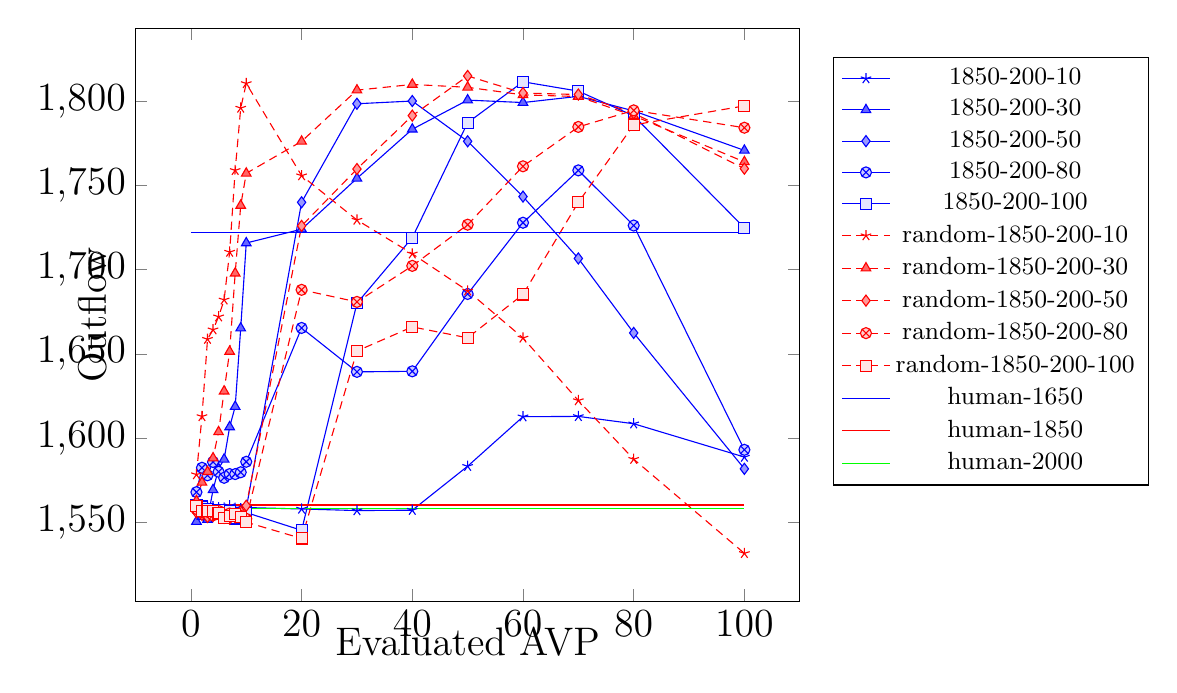
\begin{tikzpicture}[scale=1]
  \pgfplotsset{
      scale only axis,
      every x tick label/.append style={font=\Large},
      every y tick label/.append style={font=\Large},
	legend style={at={(1.05,0.95)},anchor=north west}
  }

\pgfplotscreateplotcyclelist{mycolorlist}{%
	blue,every mark/.append style={fill=blue!80}, mark=star, error bars/.cd, y dir=both, y explicit\\%
	blue,every mark/.append style={fill=blue!60}, mark=triangle*, error bars/.cd, y dir=both, y explicit\\%
	blue,every mark/.append style={fill=blue!40}, mark=diamond*, error bars/.cd, y dir=both, y explicit\\%
	blue,every mark/.append style={fill=blue!20}, mark=otimes*, error bars/.cd, y dir=both, y explicit\\%
	blue,every mark/.append style={fill=blue!10}, mark=square*, error bars/.cd, y dir=both, y explicit\\%
	red,densely dashed,every mark/.append style={solid,fill=red!80}, mark=star, error bars/.cd, y dir=both, y explicit\\%
	red,densely dashed,every mark/.append style={solid,fill=red!60},mark=triangle*, error bars/.cd, y dir=both, y explicit\\%
	red,densely dashed,every mark/.append style={solid,fill=red!40},mark=diamond*, error bars/.cd, y dir=both, y explicit\\%
	red,densely dashed,every mark/.append style={solid,fill=red!20}, mark=otimes*, error bars/.cd, y dir=both, y explicit\\%
	red,densely dashed,every mark/.append style={solid,fill=red!10}, mark=square*, error bars/.cd, y dir=both, y explicit\\%
	green!40!black, dashed,every mark/.append style={solid,fill=green!80}, mark=star, error bars/.cd, y dir=both, y explicit\\%
	green!40!black, dashed,every mark/.append style={solid,fill=green!60},mark=triangle*, error bars/.cd, y dir=both, y explicit\\%
	green!40!black, dashed,every mark/.append style={solid,fill=green!40},mark=diamond*, error bars/.cd, y dir=both, y explicit\\%
	green!40!black, dashed,every mark/.append style={solid,fill=green!20},mark=otimes*, error bars/.cd, y dir=both, y explicit\\%
	green!40!black, dashed,every mark/.append style={solid,fill=green!10},mark=square*, error bars/.cd, y dir=both, y explicit\\%
	black, dashed,every mark/.append style={solid,fill=green!80}, mark=star, error bars/.cd, y dir=both, y explicit\\%
	black, dashed,every mark/.append style={solid,fill=green!60},mark=triangle*, error bars/.cd, y dir=both, y explicit\\%
	black, dashed,every mark/.append style={solid,fill=green!40},mark=diamond*, error bars/.cd, y dir=both, y explicit\\%
	black, dashed,every mark/.append style={solid,fill=green!20},mark=otimes*, error bars/.cd, y dir=both, y explicit\\%
	black, dashed,every mark/.append style={solid,fill=green!10},mark=square*, error bars/.cd, y dir=both, y explicit\\%
	}


\begin{axis}[
    legend style={font=\small},
	ylabel={\Large Outflow},
	x label style={at={(axis description cs:0.5,-0.03)},anchor=north},
	y label style={at={(axis description cs:-0.030,0.5)}, anchor=south},
	xlabel={\Large Evaluated AVP},
	cycle list name=mycolorlist
]

\addplot table [x=a, y=b] {
a	 b	 c
1	1559.63	13.88
2	1559.48	13.84
3	1559.05	13.82
4	1559.38	13.8
5	1558.76	14.04
6	1558.58	14.28
7	1559.95	13.46
8	1558.51	13.91
9	1558.19	13.29
10	1558.87	14.51
20	1558.01	14.14
30	1557.07	14.55
40	1557.29	14.58
50	1583.39	18.89
60	1612.76	17.66
70	1612.94	17.99
80	1608.59	19.57
100	1588.82	19.68
};
\label{1850-200-10}

\addplot table [x=a, y=b] {
a	 b	 c
1	1550.56	20.68
2	1553.54	24.55
3	1551.78	25.46
4	1569.35	25.76
5	1581.95	26.39
6	1587.49	20.18
7	1606.68	26.91
8	1618.74	29.18
9	1665.32	32.67
10	1715.83	33.37
20	1724.0	42.85
30	1754.17	46.62
40	1783.33	46.98
50	1800.61	46.48
60	1799.17	42.55
70	1802.84	37.3
80	1794.2	39.43
100	1770.77	34.31
};
\label{1850-200-30}

\addplot table [x=a, y=b] {
a	 b	 c
1	1557.22	13.75
2	1557.47	14.27
3	1556.14	14.45
4	1554.95	13.81
5	1555.7	14.04
6	1555.02	14.29
7	1553.22	11.95
8	1554.52	14.07
9	1554.41	13.74
10	1558.26	17.94
20	1739.99	36.44
30	1798.45	46.73
40	1800.07	35.4
50	1776.17	29.93
60	1743.37	26.96
70	1706.65	25.72
80	1662.48	29.64
100	1581.84	27.82
};
\label{1850-200-50}

\addplot table [x=a, y=b] {
a	 b	 c
1	1567.98	14.71
2	1582.45	18.75
3	1577.99	20.42
4	1585.91	17.36
5	1580.08	17.9
6	1576.51	14.79
7	1578.71	16.52
8	1578.71	15.65
9	1579.79	15.35
10	1586.02	23.28
20	1665.43	24.45
30	1639.37	29.93
40	1639.69	37.21
50	1685.59	48.49
60	1727.86	51.61
70	1758.92	38.4
80	1726.2	38.14
100	1593.11	30.61
};
\label{1850-200-80}

\addplot table [x=a, y=b] {
a	 b	 c
1	1560.35	15.74
2	1559.48	16.46
3	1557.9	15.84
4	1556.89	16.4
5	1557.58	15.84
6	1553.36	17.84
7	1556.89	17.19
8	1552.39	16.42
9	1555.45	17.76
10	1555.88	17.41
20	1545.34	17.78
30	1680.08	25.0
40	1719.0	38.13
50	1787.22	56.02
60	1811.48	37.64
70	1805.94	31.41
80	1791.29	29.53
100	1724.83	27.83
};
\label{1850-200-100}

\addplot table [x=a, y=b] {
a	 b	 c
1	1578.42	16.21
2	1612.91	18.97
3	1658.77	23.5
4	1664.39	21.81
5	1672.09	22.83
6	1682.1	23.34
7	1710.47	32.95
8	1758.96	33.62
9	1795.93	31.41
10	1810.51	28.73
20	1755.79	38.14
30	1729.48	36.16
40	1709.42	42.36
50	1687.46	35.91
60	1659.49	41.28
70	1622.38	54.02
80	1587.56	56.24
100	1531.69	56.26
};
\label{random-1850-200-10}

\addplot table [x=a, y=b] {
a	 b	 c
1	1562.83	15.83
2	1573.78	15.35
3	1580.08	17.19
4	1588.21	20.74
5	1603.73	18.79
6	1627.88	22.59
7	1651.46	26.07
8	1697.9	31.4
9	1738.12	27.42
10	1757.16	26.37
20	1776.13	47.77
30	1806.52	43.19
40	1809.9	41.44
50	1808.21	30.71
60	1803.71	33.3
70	1802.74	30.27
80	1791.32	25.59
100	1763.96	26.64
};
\label{random-1850-200-30}

\addplot table [x=a, y=b] {
a	 b	 c
1	1556.03	13.05
2	1554.52	14.18
3	1553.26	14.09
4	1553.9	13.38
5	1555.63	14.08
6	1552.79	15.65
7	1552.25	16.07
8	1553.04	16.82
9	1556.46	15.41
10	1559.92	16.29
20	1725.98	37.02
30	1759.72	53.04
40	1791.4	44.49
50	1814.94	38.71
60	1804.82	37.74
70	1803.92	31.76
80	1792.87	27.42
100	1759.93	27.77
};
\label{random-1850-200-50}

\addplot table [x=a, y=b] {
a	 b	 c
1	1557.97	14.18
2	1556.03	13.19
3	1556.32	13.31
4	1554.23	14.68
5	1556.86	15.02
6	1553.54	12.27
7	1555.31	14.88
8	1554.3	16.09
9	1553.98	14.08
10	1552.21	16.42
20	1688.04	24.67
30	1680.88	36.8
40	1702.26	50.61
50	1726.7	51.5
60	1761.34	56.24
70	1784.7	50.65
80	1794.53	40.4
100	1784.23	28.79
};
\label{random-1850-200-80}

\addplot table [x=a, y=b] {
a	 b	 c
1	1559.59	15.06
2	1556.82	12.66
3	1556.82	16.25
4	1556.57	14.51
5	1555.34	13.48
6	1552.64	14.58
7	1553.69	14.2
8	1554.84	14.1
9	1553.04	15.07
10	1550.2	14.54
20	1540.51	16.07
30	1651.75	28.07
40	1666.04	23.78
50	1659.56	30.07
60	1685.3	41.46
70	1739.95	47.67
80	1785.89	64.6
100	1797.19	26.94
};
\label{random-1850-200-100}

\addplot[blue, samples=200] coordinates {(0,1722.200000) (100,1722.200000)};\label{human-1650}\addplot[red, samples=200] coordinates {(0,1560.380000) (100,1560.380000)};\label{human-1850}\addplot[green, samples=200] coordinates {(0,1558.120000) (100,1558.120000)};\label{human-2000}\addlegendimage{/pgfplots/refstyle=1850-200-10}
\addlegendentry{1850-200-10}
\addlegendimage{/pgfplots/refstyle=1850-200-30}
\addlegendentry{1850-200-30}
\addlegendimage{/pgfplots/refstyle=1850-200-50}
\addlegendentry{1850-200-50}
\addlegendimage{/pgfplots/refstyle=1850-200-80}
\addlegendentry{1850-200-80}
\addlegendimage{/pgfplots/refstyle=1850-200-100}
\addlegendentry{1850-200-100}
\addlegendimage{/pgfplots/refstyle=random-1850-200-10}
\addlegendentry{random-1850-200-10}
\addlegendimage{/pgfplots/refstyle=random-1850-200-30}
\addlegendentry{random-1850-200-30}
\addlegendimage{/pgfplots/refstyle=random-1850-200-50}
\addlegendentry{random-1850-200-50}
\addlegendimage{/pgfplots/refstyle=random-1850-200-80}
\addlegendentry{random-1850-200-80}
\addlegendimage{/pgfplots/refstyle=random-1850-200-100}
\addlegendentry{random-1850-200-100}
\addlegendimage{/pgfplots/refstyle=human-1650}
\addlegendentry{human-1650}
\addlegendimage{/pgfplots/refstyle=human-1850}
\addlegendentry{human-1850}
\addlegendimage{/pgfplots/refstyle=human-2000}
\addlegendentry{human-2000}


\end{axis}
\end{tikzpicture}
\end{document}
